%!TEX root = thesis.tex
\todo{Change all names to fictional names}

\todo{purpose of workshops, why do we do it!}

Preliminary workshops were conducted to explore the design space of \todo{ad hoc interfaces} in the home environment.
The intend was to get a deeper understanding of how regular users, the participants, interact with products in their home and to explore the potential in the notion of \todo{ad hoc interfaces}.

\section{Workshop approach}
\label{ch:workshops:approach}
Our approach to the workshops was inspired by different elements from the literature. \todo{\dots}
We have not taken one specific design method approach but a more loosely structured one where inspiration from other methods have been incorporated.

The home of the participants were chosen to be the workshop setting.
This decision was made because we wanted the participants to feel comfortable and also because of the familiarity of being at home in terms of routines and \todo{etc}

\subsubsection{Obstructions}
\label{ch:workshops:approach:obstructions}

When trying to explore potential interactions and situations it can be beneficial to scope the setting by staging a concrete and limited scenario which participants can adhere to.





\todo{creating obstructions and staging the situation.}


\subsection{Props}
\label{ch:workshops:approach:props}
\todo{mangler bl.a. at bringe teori p\aa \ banen}

In preparation for the workshops we collected a variety of different props that could potentially be useful mediators during the workshops.
The intention here was to have artefacts that could spur imagination amongst the participants and help stage the fictional spaces created.

Figure~\ref{ch:workshops:props-box} shows a box with the props chosen for the workshops.

\begin{itemize}
  \item{Pen, paper(A3, A4), Post-Its, white board foil and transparencies for sketching, drawing and note-taking.}
  \item{Different fabrics like cloth and a fabric-surface mousepad for their flexible characteristics.}
  \item{Plasticine for direct manipulation and for moulding different shapes}
  \item{Rigid objects which could have imaginative behaviour and functionality.}
\end{itemize}

\begin{figure}[hb]
  \centering
    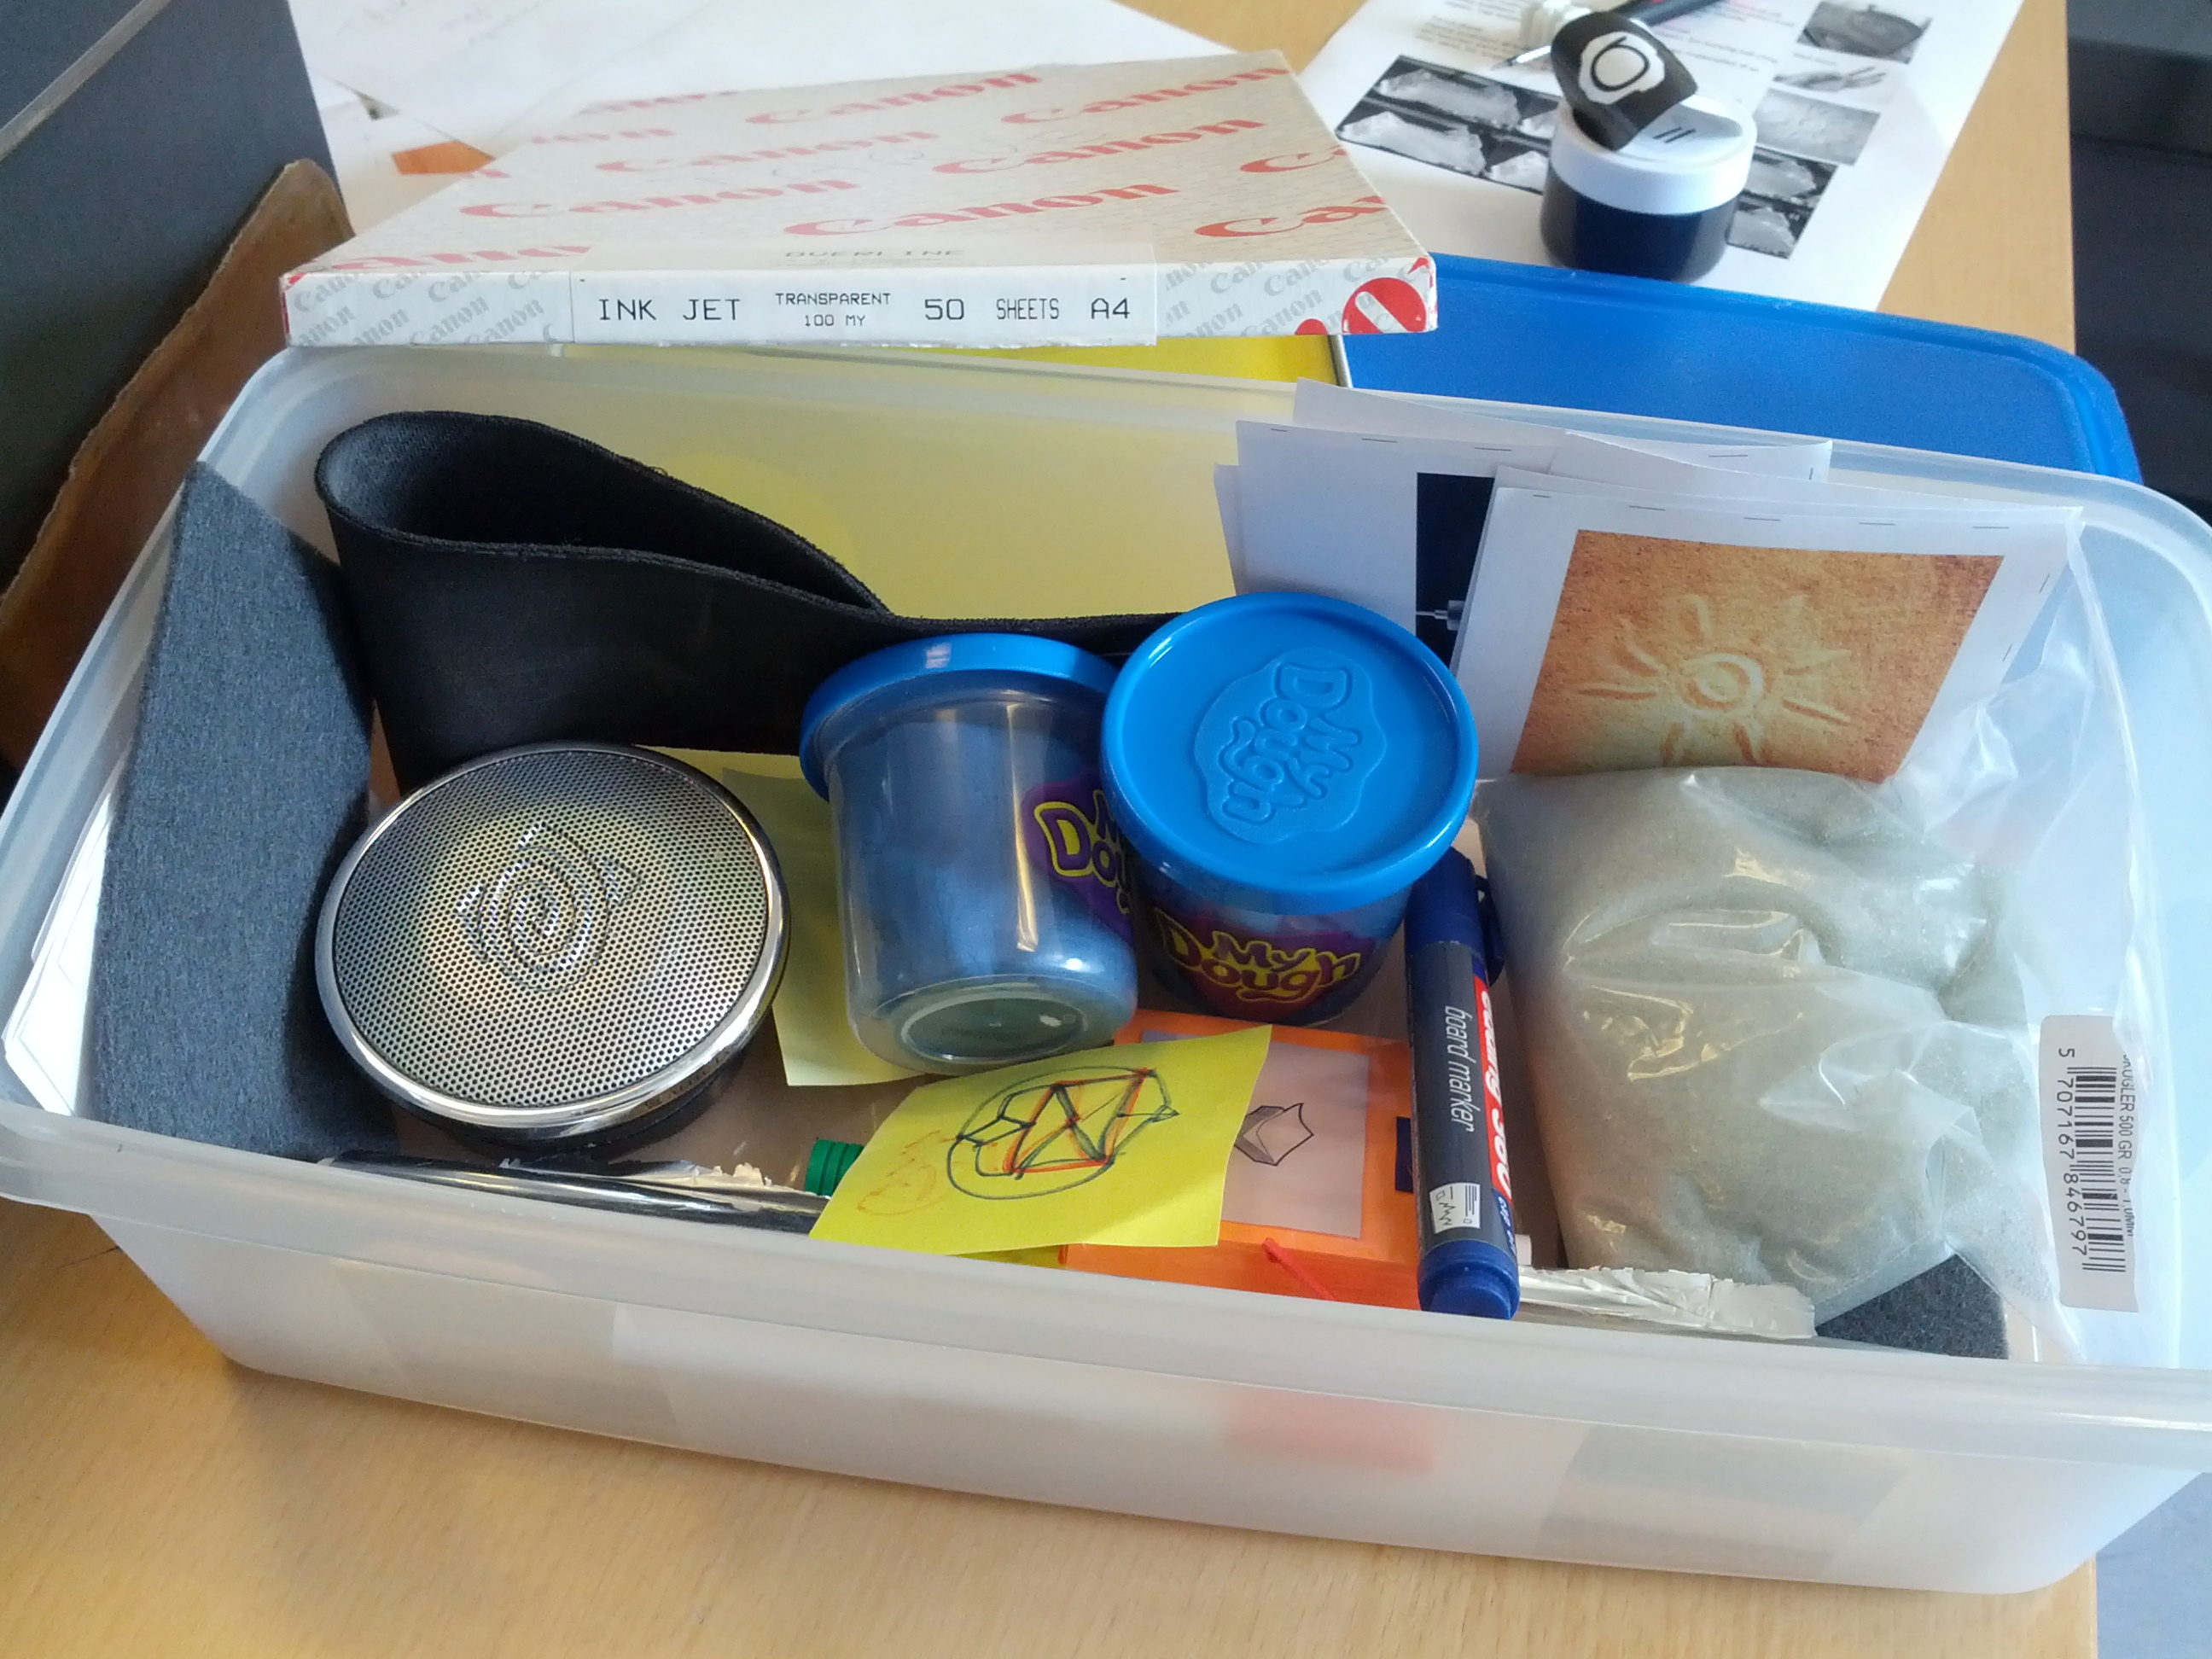
\includegraphics[width=4in]{workshops/props-box}
    \caption[A box with a variety of workshop props.] % in list of figures
  {The box with a variety of workshop props.} % beneath the figure
  \label{ch:workshops:props-box}
\end{figure}

\subsection{Workshop introduction}
\label{ch:workshops:approach:introduction}
By way of introduction, we would in both workshops sit down at a table with the participants over a cup of coffee and some chatting, as a way to set an informal atmosphere.
Subsequently we would give a brief introduction as to what was about to happen and what we would expect from them.

Following the introductory part we would start off with an opening question which could initiate the workshop discussions and scenarios:

\begin{quotation}
  \emph{What was the last thing you interacted with before you left home this morning.}
\end{quotation}

Taking on from the answer to the question, we would try to introduce the earlier mentioned obstructions in the environment.
For example, if the answer was the living room TV, one obstruction could be to eliminate the remote control and encourage the person to find other means of interacting with the device in mind (TV).
In this way we would hope to see alternative and interesting ways of interacting with devices in an ad hoc way, only with what was available in the immediate surroundings.

\todo{and by the use of props?}

\section{Workshop I}
\label{ch:workshops:workshop-i}
Our initial workshop attempt was conducted with two participants, Kristoffer and Tina Kaia, both in their mid twenties.
Kristoffer is from the same education as ourselves, ICT Product Development, and Tina Kaia is a fourth year student of anthropology.
The workshop was carried out in Tina Kaias home in Aarhus where she lives with Tore (one of the authors).
See appendix~\ref{app:workshops-i} for \todo{a transcript?? and} audio files.

A lot of this workshop was focused around the living room furniture, especially the sofa environment which is a place for relaxation and socialisation.
In this way the devices that came in to play were the ones in the direct surroundings, e.g. TV, Hi-Fi appliances and lighting.

\todo{inset billede af stuen}
\todo{what did we ask them to do}

The idea of using the sofa itself as a medium for communication between a person and the TV was brought up.
In this way a person could use the sofa as a embedded remote control through various interactions anywhere on the surface.
We experimented with different ways of interacting with the sofa but using gestures on the surface of the sofa was a recurring theme.

One idea was to move the `remote' in to the periphery, using it merely with your hand and not requiring your direct visual attention \todo{tegning eller billede}.

Another idea was add visual feedback to it through the textiles of the sofa.
We discussed an approach with plain textile sofa coating where the materiality of the textiles would provide a subtle visual feedback.
Textiles like suede, velour and synthetic textiles where touch can leave markings on the surface could potentially provide this kind of feedback.
And the inherent ability to quickly remove the markings again would be beneficial as well.

In both ideas the characteristics of an ad hoc interface are apparent; the interface is created on demand and exists only as long as needed.
As Tina Kaia puts it, when comparing the embedded sofa remote with a normal remote control

\begin{quotation}
  \emph{``\dots the interface can't disappear \dots''}
\end{quotation}
And Kristoffer adds to it
\begin{quotation}
  \emph{``\dots yeah it's forever accessible \dots it's where you are \dots''}
\end{quotation}
And later he adds
\begin{quotation}
  \emph{``\dots the cool thing is \dots they're so momentary \dots''}
\end{quotation}

Continuing on the topic of an embedded sofa remote we discussed the problems when extending it to deal with several different devices.
For example, how do we address a specific device, e.g. TV, lights or a HiFi system? and how does the system know we are addressing it?.
\blank
Being able to address multiple devices in the home creates some complications as we need a method to unambiguously address a specific device.
In comparison, a normal multi-purpose remote control could obtain unambiguous addressing through \emph{point-and-click} (direction) or \emph{select-and-click} (context button).
Different ideas came into play during the workshop: \todo{insert workshop drawings of the listed ideas}

\begin{itemize}
  \item{\textbf{Symbols}: every object or object type has a symbol.\\
        Drawing, for example, a circle to indicate the TV followed by a gesture mapping to a function.
        %This requires the construction of a language based on symbols.
  }
  \item{\textbf{Direction}: drawing a line in the direction of an object.\\
        The straight path of the line is traced and an approximation to an object close to the path is made.
        %This requires that objects are placed strategically so that ambiguity is eliminated
        %\todo{should it be mentioned that: the systems also needs to know about object positions? or is that implicit?}
  }
  \item{\textbf{Layout}: sketch the room and select device position.\\
        Sketch the frame of the room followed by pointing to a device position, which afterwards is mapped to the actual layout of the room and an approximation to the actual device position is made.
        %Contains a high degree of uncertainty
  }
  \item{\textbf{Position}: relative to your position in the room.\\
        Your position in the sofa is the centre of the room so directing your attention to a lamp on your left side would require gestures on your left side.
        %\todo{mange ting kan v\ae re til venstre for dig}
  }
\end{itemize}

Giving feedback to the user is also of a more or less complicated nature.
\todo{Moos, ``det er mig du har gang i''}
Again, when comparing to a normal remote control you do not have the inherent tactile feedback from pushing a button.
During the workshop we discussed this issue and a few suggestions where made on how to address it:
\begin{itemize}
  \item{Visual feedback on the device such as light.}
  \item{\hl{Auditory feedback from the device or elsewhere in the room} }
  \item{Haptic feedback through for example vibrations in the sofa.}
\end{itemize}

\begin{verbatim}
raised issues:
  feedback - det er mig du har gang i
\end{verbatim}

\subsection{Discussion}
\label{ch:workshops:workshop-i:discussion}

This first workshop was marked by having emphasis on the idea of a smart sofa.
The key findings was an assortment of interaction potentials which were discussed and played out with the participants.
Not all of the suggested interaction possibilities are equally good but \todo{\dots}
The idea of a smart sofa should of course not be seen as an isolated concept.
The touch technology could be extended to other furniture, objects or even walls and floors.

Because of Kristoffer's background in our field of study he was very much active in the discussions and creative in playing out scenarios.
On the other hand, Tina Kaia was having a harder time comprehending some of the technological aspects as she was more or less unfamiliar with them.
After the workshop we did a short evaluation with the participants which made it clear that Tina Kaia would have benefited from examples or references.
These references could serve as indicators of concepts to help her and others in future workshops to come to a better understanding.

\section{Workshop II}
\label{ch:workshops:workshop-ii}
Our second workshop was carried out with also two participants, Julian and Anne, both in their mid twenties.
Julian is a fifth year student at Aarhus School of Business and Anne is a nurse on maternity leave, and together they have Alma, their eight month old daughter.
The workshop took place at their apartment in Aarhus.
See appendix~\ref{app:workshops-ii} for \todo{a transcript?? and} audio files.

We did a couple things differently for the second workshop.
One thing was to prepare some inspirational cards as referential material and to encourage creative thinking.
Another was to put more weight on expressive interactions which was something that the first workshop lacked.
Before digging in to the findings and outcomes of the this second workshop we will first introduce these new initiatives.

\subsubsection{Inspirational cards}
\label{ch:workshops:workshop-ii:inspiration-cards}
Taking from lessons learned in the previous workshop about supporting disparate participants with referential material, we compiled a stack of small cards with pictures printed on them that would hopefully work as sources of inspiration.
The cards were motivated by \emph{Inspiration cards} describe in the \emph{Inspiration Card Workshops}, \citep{halskov2006inspiration}.
The \emph{Inspiration Card Workshop} is a participatory design method where designers work together with collaborators, often with a specific domain knowledge, to create new design concepts.
The method recognises that participants have a disparate background and that sources of inspiration can play an important role in the design process.
These sources are manifested in \emph{inspiration cards} on which an image and some textual information is printed.
The cards are divided in to two main categories:
\begin{itemize}
  \item{\emph{Technology cards}, which represents a specific technology or an application of one or more technologies.}
  \item{\emph{Domain cards}, which represent information on the domains within the design space.}
\end{itemize}

\todo{description of the chosen technologies and applications - we chose technologies that we saw ad hoc potential in??}

The design method is intended to be used in the early stages of a design process where designers and collaborators seek to close in on future designs.

In our workshop we have used \hl{a simplified approach to} inspirational cards as a means of communication between designers (ourselves) and the participants.
Our \emph{inspiration cards} categories have been altered compared to \citep{halskov2006inspiration} to fit our needs.
Instead of having several different domain cards we chose to see the context of the home environment as the domain and have the cards represent different common interactive appliances of the home.
Regarding technology cards, we have taken the topic of technology as a mixture of materiality and form, and interactions.
Textual descriptions on the cards were almost non existent as we did not find the need to detail the cards more than just with images.
See figures~\ref{ch:workshops:technology-cards} and \ref{ch:workshops:appliance-cards} which list the prepared inspirational cards.

The cards were created with a varying degree of conceptual distance to encourage creative thinking and diversity, \citep[chap. 10]{benyon2005designing}.
Some cards were created with metaphorical references in mind.
For example, a picture with a sun drawn in sand was added to conceptually describe something that could be affected by external factors and could fade and disappear over time.
Other cards, i.e. a picture with various gestures on a mouse pad, were conceptually close and more easily recognisable.

\subsubsection{Expressive interaction}
\todo{we tried to get the participants to engage in more expressive interactions.}


\section{Brainstorm session}
Brainstorm med Matthias


\begin{figure}
\centering
\begin{minipage}[t]{.5\textwidth}
  \centering
  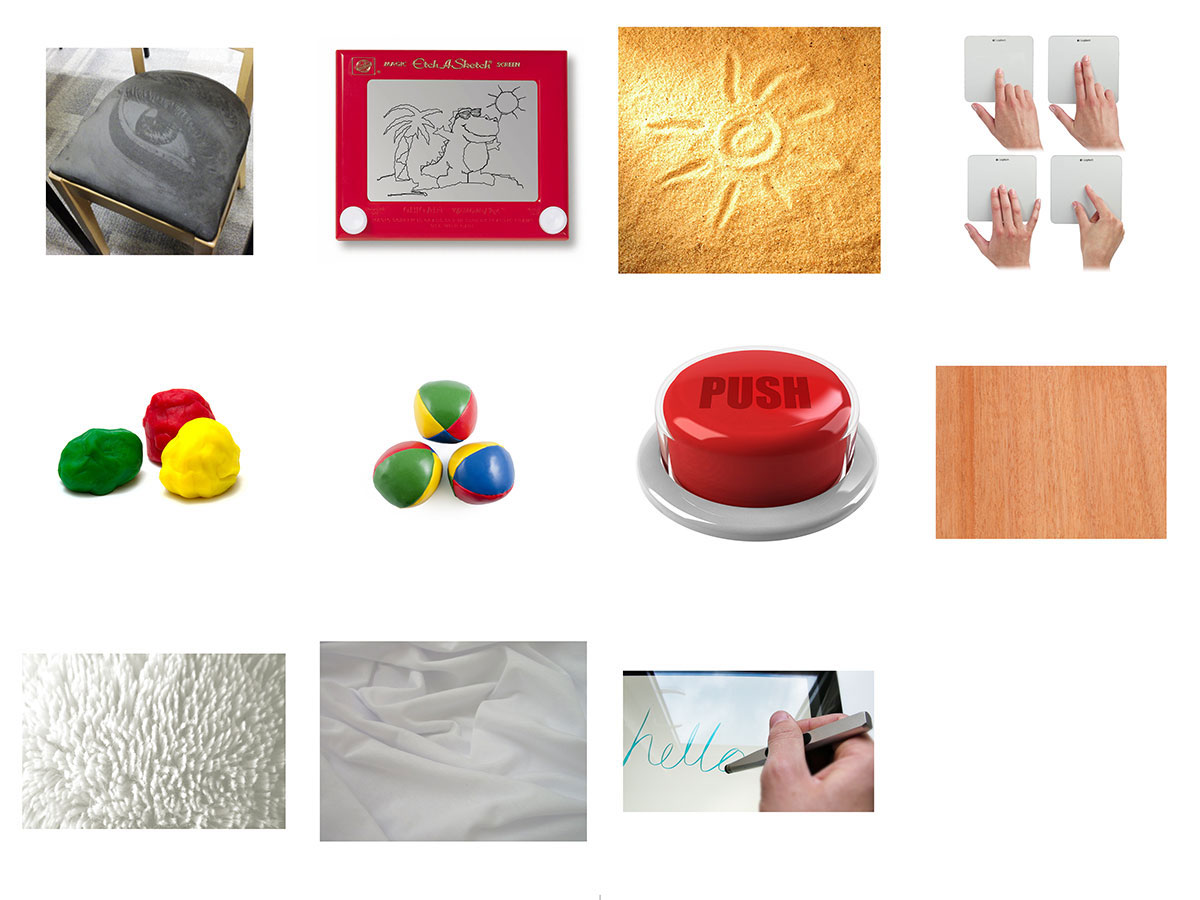
\includegraphics[width=0.9\linewidth]{workshops/technology-cards}
  \captionof{figure}{Technology cards}
  \label{ch:workshops:technology-cards}
\end{minipage}%
\begin{minipage}[t]{.5\textwidth}
  \centering
  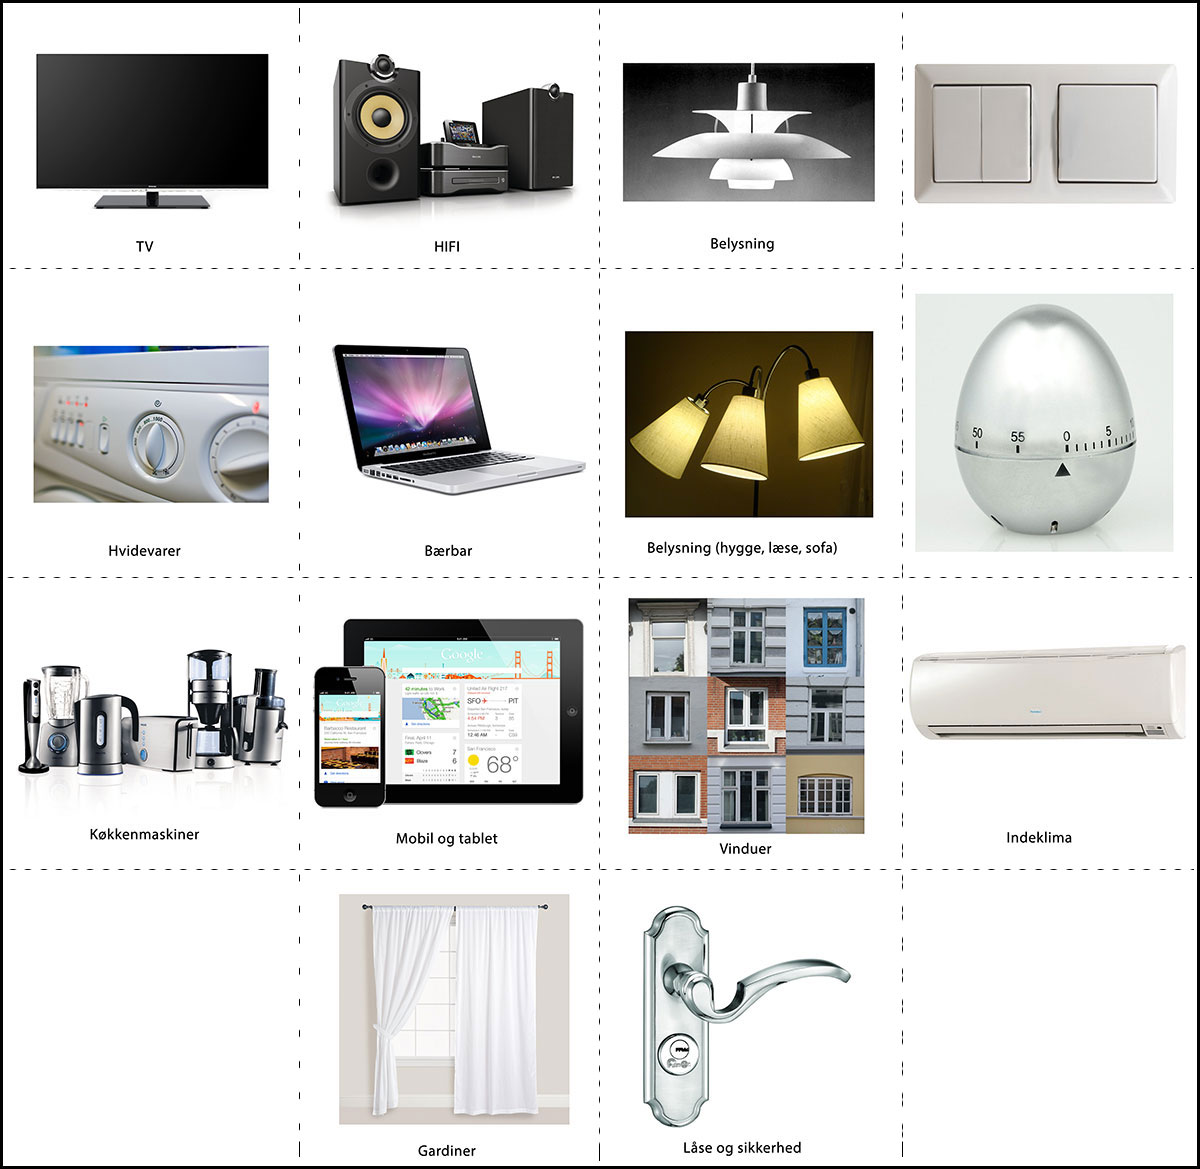
\includegraphics[width=0.9\linewidth]{workshops/appliance-cards}
  \captionof{figure}{Appliance cards}
  \label{ch:workshops:appliance-cards}
\end{minipage}
\end{figure}

\subsection{Discussion}
\label{ch:workshops:workshop-ii:discussion}

\section{Discussion}
\label{ch:workshops:discussion}

How did the workshops work as a whole. expectancies and actual findings.

\todo{Conventions and the familiarity of the home ... Dindler, 2010 - Lerdahl, Bell, Ehn...} Were we successful in defamiliarising the home setting???

\todo{summery, hvad fik vi ud af det}

